\chapter{Simulations and Results}
\label{chap:scenarios} 

This chapter will test the adaptation algorithms implemented in the \textit{ABR}
module from the \autoref{chap:abrmodule} in various simulated scenarios. The \autoref{sec:metrics}
will present the metrics used for the comparisons. The \autoref{sec:scenarios} will 
go through all the simulation scripts and its results,
analyse the performance and fairness of the adaptation algorithms. Finally, the \autoref{sec:simconclu},
will discuss the conclusions and limitations of the \textit{ABR} module.

% \section{Introduction}

\section{Comparison Metrics}
\label{sec:metrics}

For the comparison, the metrics introduced in the \autoref{sec:qoemetrics} will be used.
In addition, other metrics will be used that may also be of interest. And they are as follows:

\begin{itemize}[topsep=0pt, noitemsep]
    \item \textbf{Average Throughput}. The average of the network throughput.
    \item \textbf{Playback start time}. The time the client takes to start the playback.
    \item \textbf{Total time watched}. Total time watched by the client.
    \item \textbf{Quality switches}. The number of times the representation changed.
    \item \textbf{Paused times}. The number of times the playback paused.
    \item \textbf{Time at each quality}. The time spent at each quality.
    \item \textbf{Buffer status}. The buffer status in milliseconds of content as a function of time.
    \item \textbf{QoE Score}. This is a score based on various metrics.
    
    The QoE score is defined for this thesis in order to compare the different algorithms. It 
    ranges from 0 to 1, the greater the score the better the performance. The formula is as follows:
    \begin{equation}
        QoE\ score = \frac{t_w-pb_s-\sum_{i=1}^{M} \frac{t_i}{2}\cdot (\frac{1}{2}-\frac{i+1}{M})-\frac{1}{2}\cdot (qs+pt)}{simulation\ time}
    \end{equation}
    with
    \begin{itemize}[topsep=0pt, noitemsep]
        \item[$\circ$] $t_w$ 		                            Time watched
        \item[$\circ$] $pb_s$ 		                            Playback start time
        \item[$\circ$] $t_i\ _{q=\{0,1,...,M\}}$ 		        Time at each quality 
        \item[$\circ$] $qs$ 		                            Quality switches
        \item[$\circ$] $pt$ 		                            Paused times
    \end{itemize}

\end{itemize}

% \section{Example script}
% \label{sec:example}


\section{Scenarios}
\label{sec:scenarios}

In the next sections, the throughput rule of \textit{dash.js} will be refered as \textit{DASH throughput},
the BOLA rule as \textit{BOLA}, the bandwidth estimation of \textit{hls.js} as \textit{HLS} and the combination
of the BOLA and the throughput rule of \textit{dash.js} simply as \textit{DASH}.

\subsection{Scenario 1}
This section will take a look a basic network scenario. To be as simply as possible, the will be 
only two nodes linked with a \texttt{PointToPoint} connection. The simulation time is 50 seconds 
and the datarate will vary in time. In this scenario, seven bitrates are used.

\begin{figure}[h]
    \centering
    % 
\includegraphics[width=0.3\textwidth]{img/space.png}
    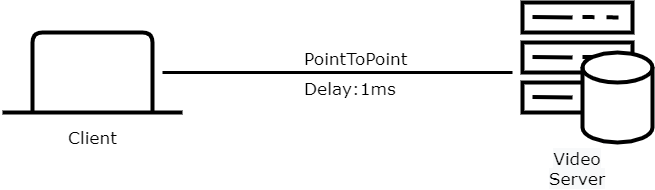
\includegraphics[width=0.45\textwidth]{img/scenario1.png}
    \caption{Scenario 1}
    \label{fig:scenario1}
\end{figure}

\begin{figure}[]
    \centering
    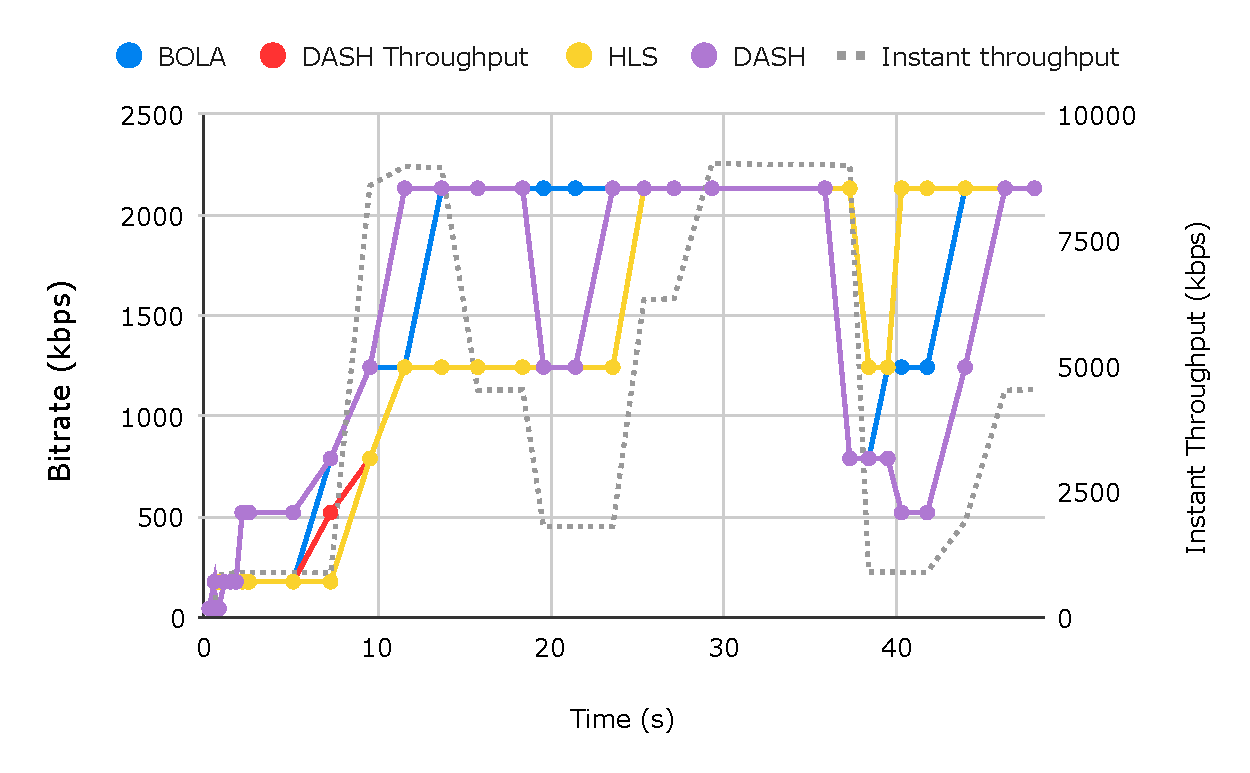
\includegraphics[width=\textwidth]{img/s1c1_1.pdf}
    \caption{Scenario 1. Quality vs time}
    \label{fig:s1c1}
\end{figure}

By looking at the \autoref{fig:s1c1}, the first thing noticeable is that the \textit{HLS} and the \textit{DASH throughput}'s
quality functions are almost the same line. \textit{BOLA} reached a little bit earier to the quality index 5 and 
sustained a good overall performance.
The combination of both rules in \textit{DASH} seems to work pretty nicely, with one exception of going
down to quality index 2 almost at the end of the simulation. 

\begin{figure}[]
    \centering
    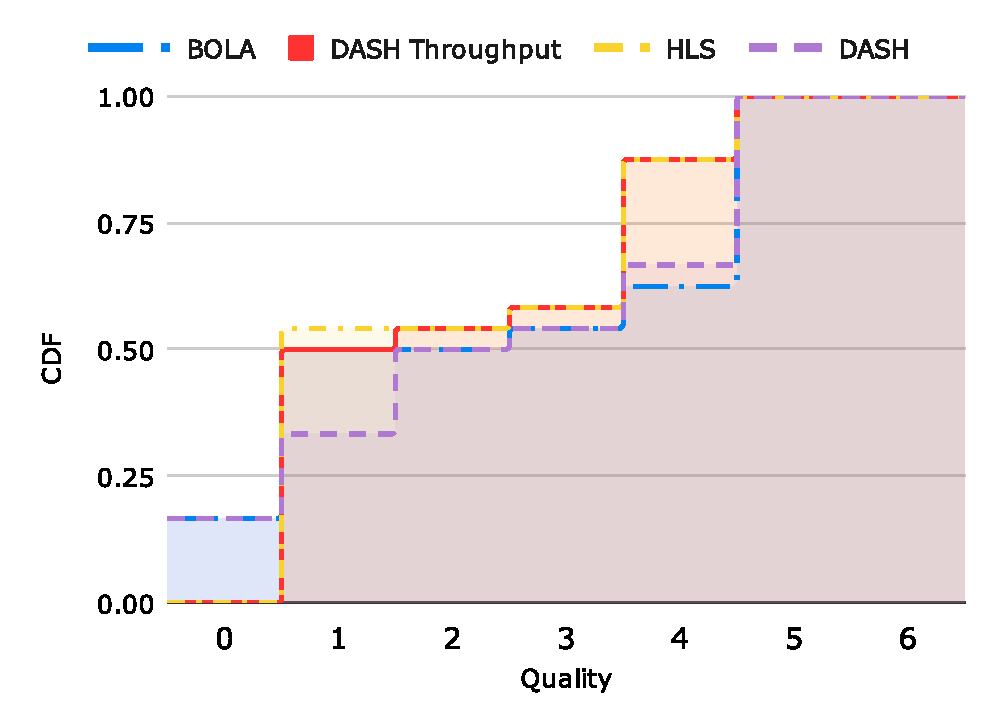
\includegraphics[width=0.8\textwidth]{img/s1c2.pdf}
    \caption{Scenario 1. CDF quality}
    \label{fig:s1c2}
\end{figure}

The \autoref{fig:s1c2} show a \textit{Cumulative Distribution Function (CDF)}. In this 
case, the \textit{CDF} shows the video quality choice statistics in the form of percentages. 
Both \textit{HLS} and \textit{DASH throughput} obteined a higher quality during most of 
the simulation time and never played segments from the lowest quality.

\clearpage

\subsection{Scenario 2}

\begin{figure}[h]
    \centering
    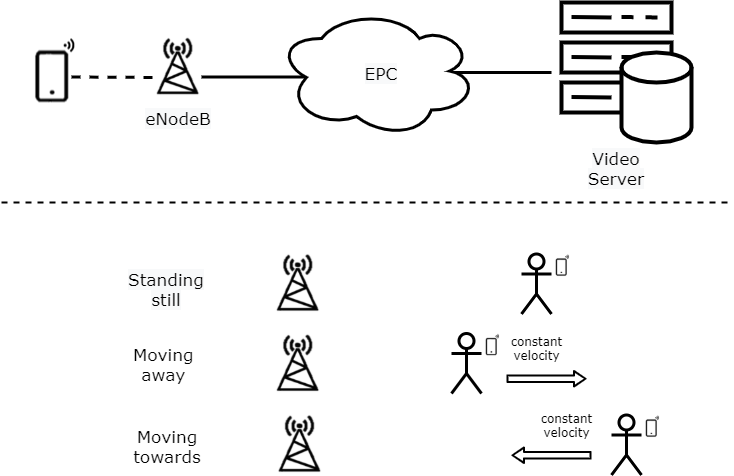
\includegraphics[width=\textwidth]{img/scenario2.png}
    \caption{Scenario 2}
    \label{fig:scenario2}
\end{figure}

This scenario will find out what will happen if an \textit{UE} stands still, or if it is moving away
or towards the \textit{eNodeB}. The only changing factor is the position of the \textit{UE}, 
the rest of the parameter remains the same. There are only one \textit{eNodeB}, meaning there 
is no possibility to handover.

This setup will be using only the \textit{HLS} algorithm. In the first simulation, the \textit{UE}
will be placed at a reasonable distance from the \textit{eNodeB}. In the second one, the \textit{UE}
is moving with a constant velocity away from the \textit{eNodeB}. Finally, the \textit{UE} is placed 
a little bit further and walks towards the \textit{eNodeB}.


The \autoref{fig:s2c1} shows the buffer status as a function of time. What moving away from 
the \textit{eNodeB} really does is to decrease the available bandwidth and finally the \textit{UE}
will be unable to request a new segment. 

Within the wireshark statistics tools, by selecting the throughput option within \textit{TCP} flows, 
it is possible to display throughput graphs of the \textit{UEs}. In the \autoref{fig:s2c2}, the first
graph show that the \textit{UE} approaching the \textit{eNodeB} performs relatively well. By contrast,
the throughput of the second \textit{UE} drops significantly every time it goes further from the \textit{eNodeB}.
All 
\begin{figure}[h]
  \centering
  
\includegraphics[width=\textwidth]{img/space.png}
  
\includegraphics[width=\textwidth]{img/space.png}
  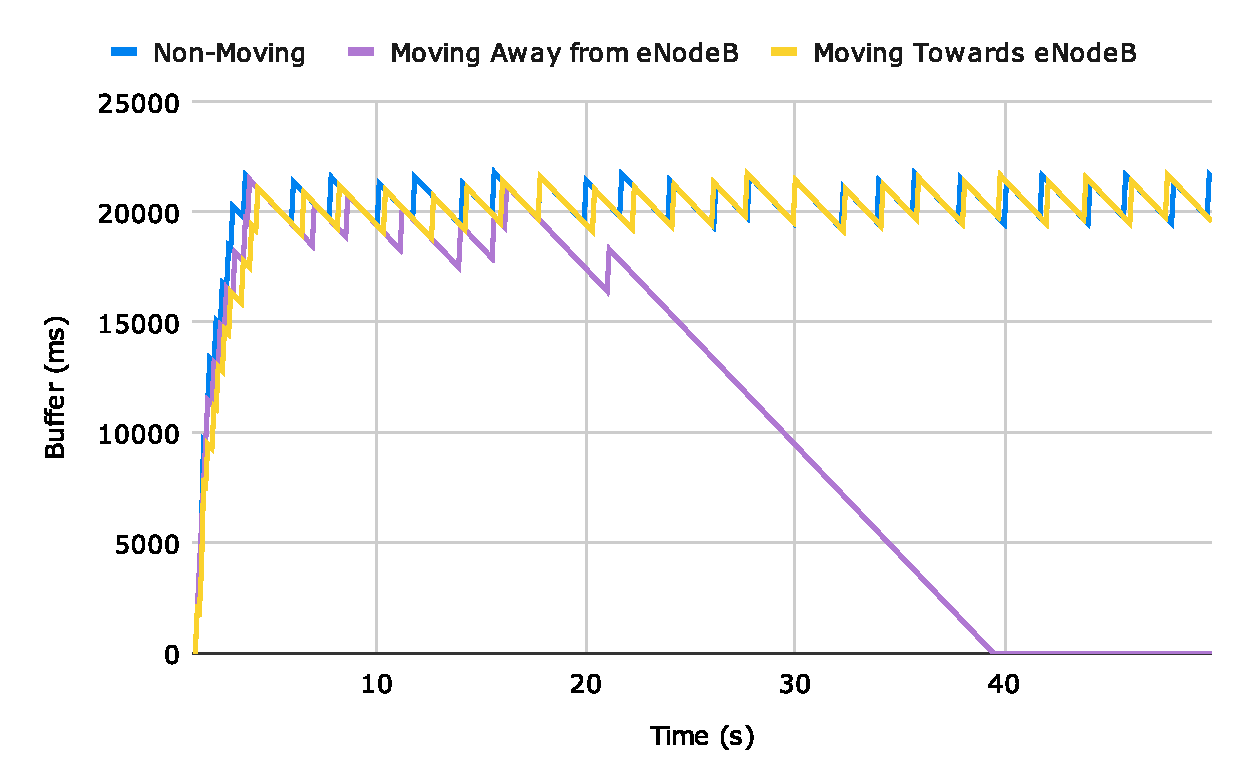
\includegraphics[width=\textwidth]{img/s2c1.pdf}
  \caption{Scenario 2. Buffer Status}
  \label{fig:s2c1}
\end{figure}


\begin{figure}[h]
    \centering    
    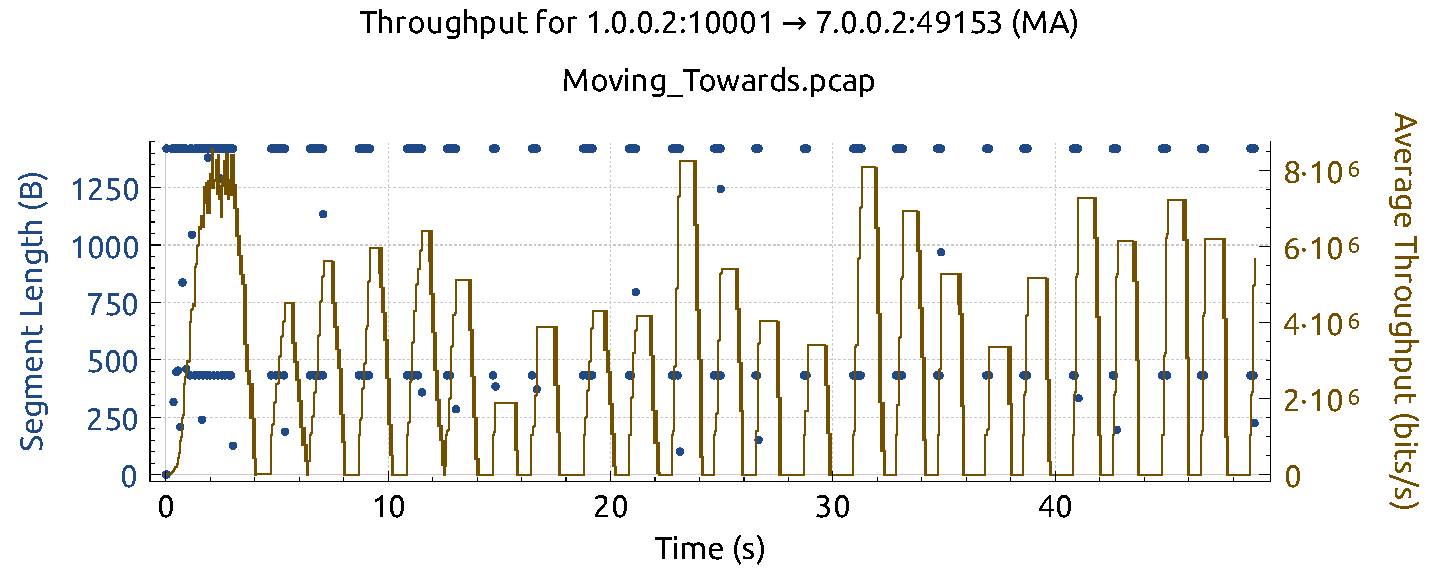
\includegraphics[width=\textwidth]{img/s2c2_1.pdf}
    
\includegraphics[width=\textwidth]{img/space.png}
    
\includegraphics[width=\textwidth]{img/space.png}
    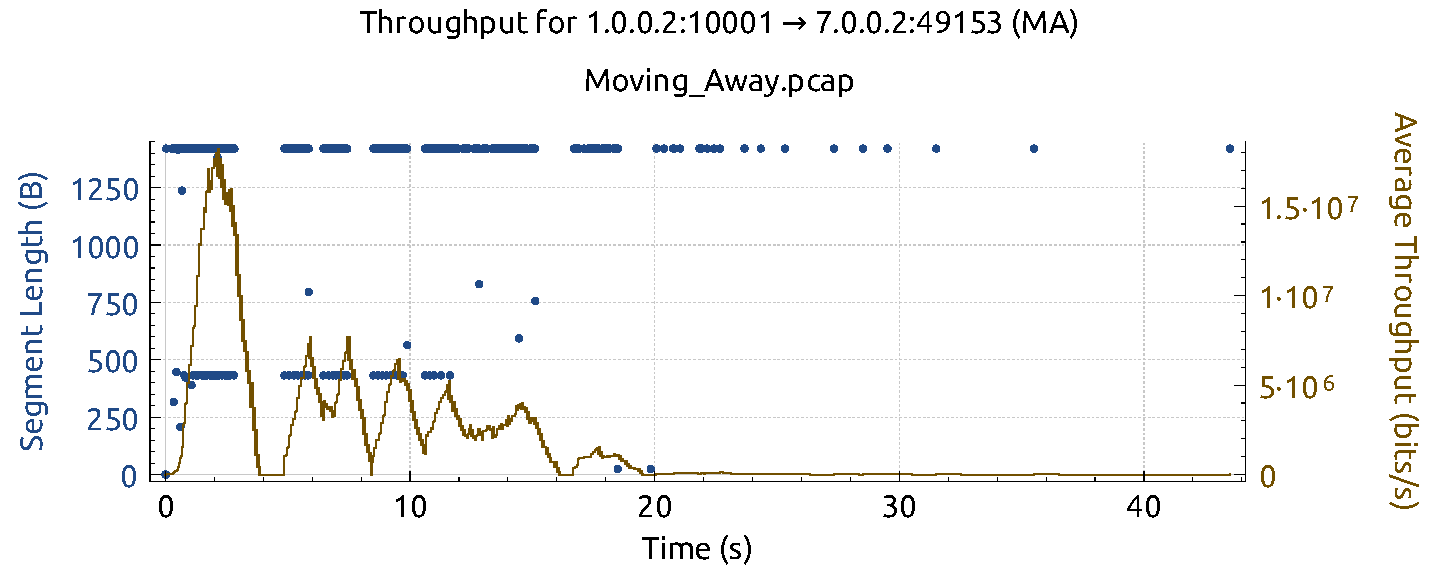
\includegraphics[width=\textwidth]{img/s2c2_2.pdf}
    \caption{Scenario 2. Throughput}
    \label{fig:s2c2}
\end{figure}


\begin{table}[]
    \centering
    \begin{tabular}{@{}llll@{}}
    \toprule
                              & Non-Moving & Moving Away & Moving Towards \\ \midrule
    QoE Score                 & 0.812078   & 0.535326    & 0.701826       \\
    Average throughput (Mbps) & 23.0487    & 8.1720      & 12.7028        \\
    Time watched (s)          & 48.9       & 38.0        & 48.485         \\
    Quality switches          & 7          & 12          & 13             \\ \bottomrule
    \end{tabular}
    \caption{Scenario 2. Metrics Comparison}
    \label{table:s2t1}
\end{table}

\clearpage

\subsection{Scenario 3}


This section provides an analysis of a \textit{LTE} scenario with poor conditions. There will be six \textit{UEs} watching video at the same time.
three of them remain stationary and the remaining three are randomly moving.
In this scenario, fifteen bitrates are used.
The only changing factor is the position of some \textit{UEs}, 
the rest of the parameter remains the same. There are only one \textit{eNodeB}, meaning there 
is no possibility to handover.
\begin{table}[h]
  \begin{tabular}{@{}llrrrr@{}}
  \toprule
  &         & \multicolumn{1}{l}{BOLA} & \multicolumn{1}{l}{DASH} & \multicolumn{1}{l}{DASH throughput} & \multicolumn{1}{l}{HLS} \\ \midrule
  \multirow{3}{*}{QoE Score} & Average & 0.3222501667             & 0.3389108333             & 0.3891433333                        & 0.3908161667            \\
                             & Max     & 0.47895                  & 0.568955                 & 0.621531                            & 0.631055                \\
                             & Min     & 0.245517                 & 0.245722                 & 0.220542                            & 0.231055                \\ \bottomrule
  \end{tabular}
  \caption{Scenerio 3. QoE Score}
  \label{table:s3t1}
\end{table}

\begin{figure}[h]
  \centering
  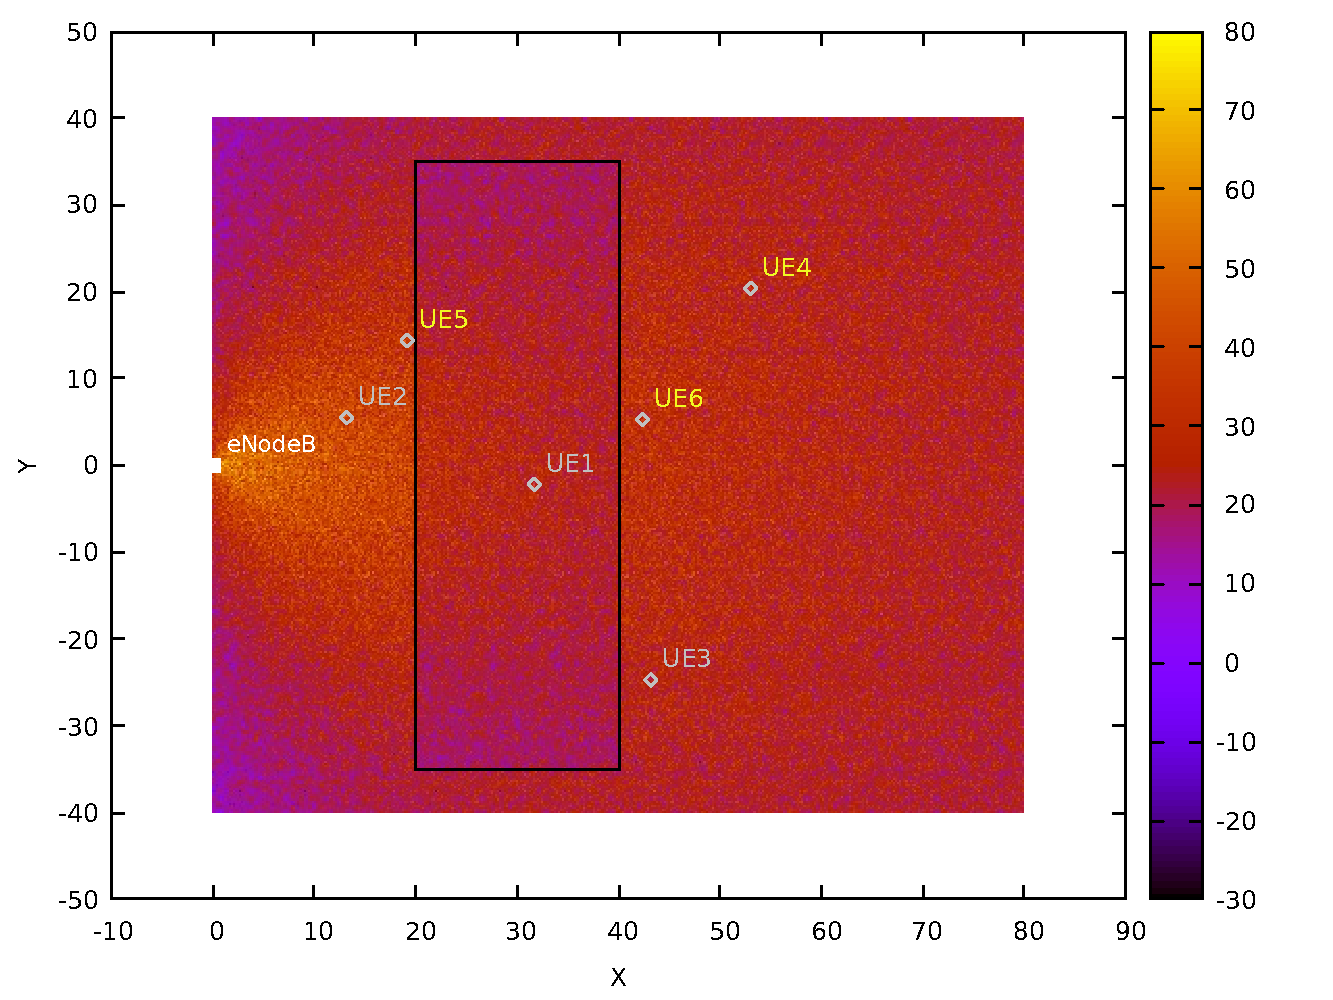
\includegraphics[width=0.97\textwidth]{img/s3i1.pdf}
  \caption{Scenario 3. Radio Environment Map}
  \label{fig:s3i1}
\end{figure}


The scenario has one \textit{eNodeB}, with one antenna, and a residential building. The 
\autoref{fig:s3i1} shows a radio enviroment map of the scenario.



With the results shown in the \autoref{table:s3t1}, we conclude that on average,
the bandwidth based algorithms have higher \textit{QoE} scores. But the other two
algorithms have less difference between their highest and lowest scores.

\clearpage

\subsection{Scenario 4}

\subsubsection{Jain Fairness Index}

Fairness metrics are used to determine whether the adaptation 
algorithm is able to deliver an equitable share of the network bandwidth 
to different clients. In this analysis, the \textit{Jain Fairness Index (JFI)}
\cite{jfi} is used. The \textit{JFI} is calculated by this formula:

% \begin{figure}[h]
%   \centering
%   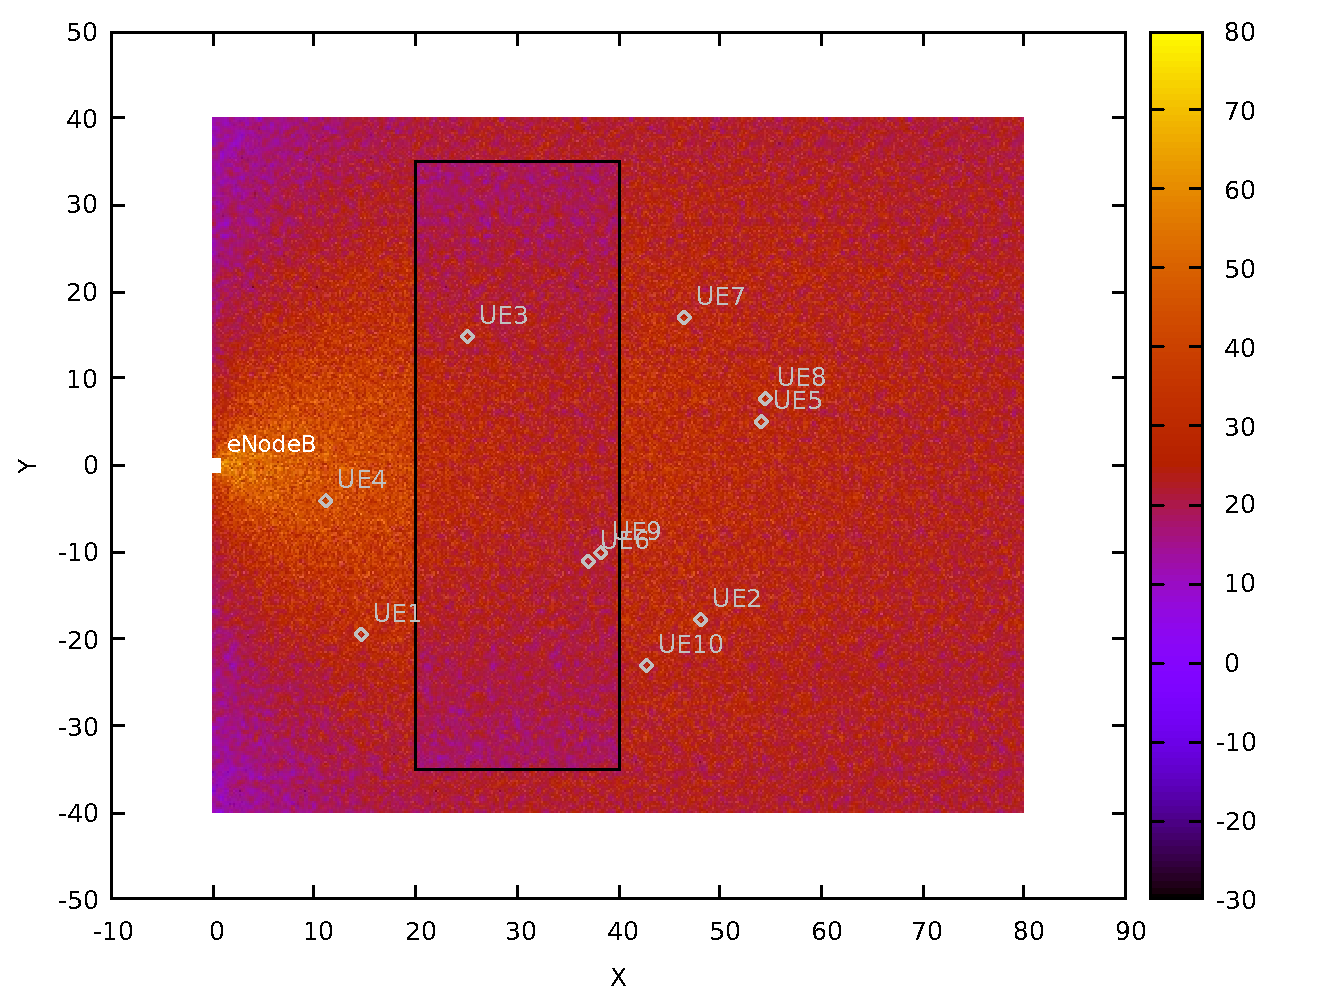
\includegraphics[width=0.95\textwidth]{img/s4i1.pdf}
%   \caption{Scenario 4. Radio Environment Map}
%   \label{fig:s4i1}
% \end{figure}

\begin{equation}
    JFI=\frac{\bigg(\sum\limits_{c\in C}\bar{B}\bigg)^2}{\left | C \right |\sum\limits_{c\in C}(\bar{B})^2}
\end{equation}

where  $C$ are the Clients and $\bar{B}$ are the Average Throughputs


\begin{figure}[h]
  \centering
  
\includegraphics[width=0.9\textwidth]{img/space.png}
  
\includegraphics[width=0.9\textwidth]{img/space.png}
\end{figure}

This testing scenario uses ten \textit{UEs} and one \textit{eNodeB} at a time in a \textit{LTE} environment.

Based on the results presented in the \autoref{table:s4t1}, the throughput based algorithms 
have the least fairness index. That is as expected seeing the results of the last scenario
because they had greater differences of performance between \textit{UEs}. That is also true in
this case, with \textit{HLS} having the single highest throughput. Nevertheless, all the
the algorithms are in a very resonable range, greater than 0.9.


\begin{figure}[h]
  \centering
  
\includegraphics[width=0.9\textwidth]{img/space.png}
  
\includegraphics[width=0.9\textwidth]{img/space.png}
\end{figure}


\begin{table}[h]
    \centering
    \begin{tabular}{@{}lrrrr@{}}
    \toprule
        & \multicolumn{1}{l}{BOLA} & \multicolumn{1}{l}{DASH} & \multicolumn{1}{l}{DASH throughput} & \multicolumn{1}{l}{HLS} \\ \midrule
    JFI & \textbf{0.972185193}     & 0.9716453768             & 0.9271291449                        & 0.929252551             \\
    MAX & 10289.8                  & 10289.8                  & 19953.9                             & \textbf{20006.4}        \\ \bottomrule
    \end{tabular}
    \caption{Scenerio 4. Fairness Comparison}
    \label{table:s4t1}
\end{table}


% \clearpage
\begin{figure}[h]
  \centering
  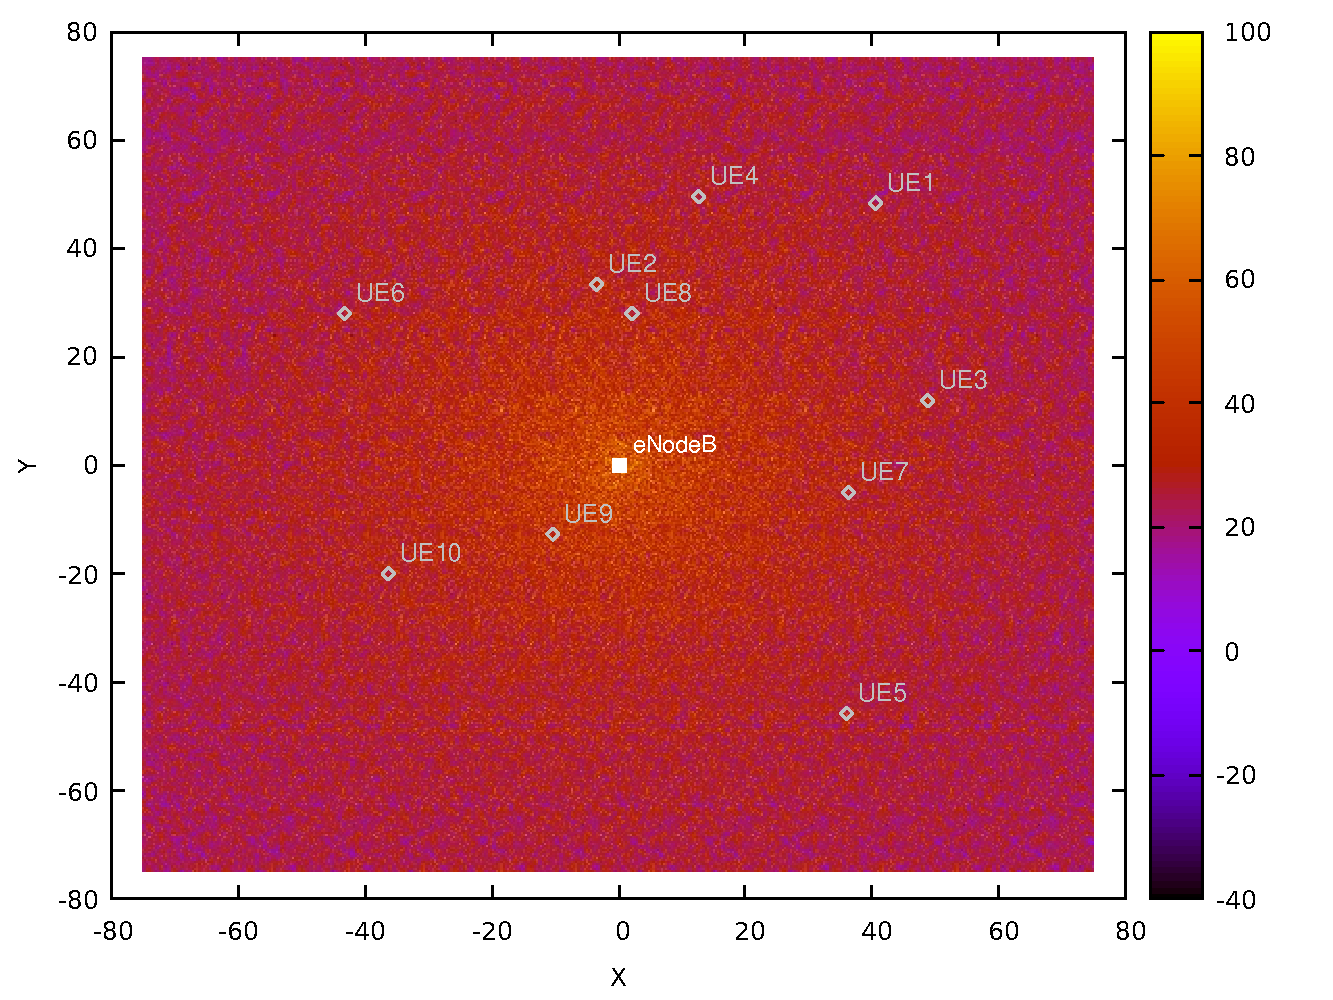
\includegraphics[width=\textwidth]{img/s4i2.pdf}
  \caption{Scenario 4. Radio Environment Map}
  \label{fig:s4i2}
\end{figure}



\clearpage

\section{Conclusions}
\label{sec:simconclu}

These testing scenarios are only a small part of what the \textit{ABR} module can do with \textit{ns-3}.
All the implemented adaptation algorithms are compered in some interesting cases. But more importantly
is to show the potential of this module and also the improvement that can be made. 

Due to limitations with \textit{ns-3}, the BOLA implementation is not complete. There some 
bugs like enabling REM will crush the simulation but the output of the REM is done without
problems. Or sometimes the simulations stops caused by some internal data structure corruption.

The implementation of BOLA was a really challenging task for this project, and its complexity 
translates, in some cases, in better performance.